\subsection{Mesher}
\label{sec:modules_mesher}
Il \emph{mesher} è il componente che, a partire dai dati forniti dal \emph{miller}, crea la mesh 3D dell'oggetto lavorato. Le interfacce verso il \emph{mesher} e verso il modulo che visualizzerà la scena sono definite: questo permette la scrittura di \emph{mesher} differenti che possono venir scelti all'avvio del software, ad esempio per visualizzare i voxel non cancellati, piuttosto che una ricostruzione del taglio eseguito, attraverso l'algoritmo Marching Cubes. Tale algoritmo viene descritto in sezione \ref{mcalgo}.

La mesh è costruita con gli strumenti messi a disposizione dalla libreria \osg: si tratterà quindi di un albero sui cui rami e sulle cui foglie sono contenute tutte le informazioni necessarie alla visualizzazione del solo oggetto lavorato. Per la struttura dell'albero si è scelto nuovamente un octree non bilanciato in cui le foglie, stavolta, contengono una molteplicità di voxel: quando il numero di oggetti contenuti in una foglia raggiunge un valore di soglia, viene aggiunto un nuovo livello all'albero, ripartendo tra i nuovi figli così creati il volume di competenza e i voxel ivi contenuti.

Il processo di \emph{meshing} si articola in due fasi: una prima fase di aggiornamento dell'albero della scena e una seconda fase in cui vengono calcolate le mesh vere e proprie. Una volta acquisiti i dati dal \emph{miller}, nella prima fase il \emph{mesher} provvede ad aggiornare la struttura eliminando tutti i voxel non più necessari ed inserendo quelli nuovi o modificati, a patto che siano visibili (vengono cioè ignorate tutte le informazioni riguardanti volumi strettamente interni alla superficie dell'oggetto lavorato). \'E importante notare che le informazioni manipolate in questa prima fase sono strettamente legate ai voxel contenuti nell'octree del \emph{miller} e vengono salvate in uno ``spazio utente'' messo a disposizione dagli oggetti di \osg. Ciò permette di ottenere una complessità computazionale $O(1)$ in cancellazione e aggiornamento e tendente a $O(\log_{8}(\text{\# voxel da visualizzare}/\text{max voxel per foglia}))$ per l'inserimento. L'albero così arricchito di informazioni aggiuntive viene quindi ritornato e, al momento della visualizzazione, scatta la seconda fase di \emph{meshing}: per ciascuna foglia modificata nella fase precedente viene ora creata una mesh vera e propria, contenente tutte le informazioni dei voxel di competenza della foglia stessa. Questa scelta permette di ottimizzare l'uso delle risorse grafiche in quanto limita l'estensione dell'albero della scena e diminuisce il numero di mesh da rappresentare, aumentandone la dimensione.

\subsubsection{L'algoritmo Marching Cubes}
\label{mcalgo} Marching Cubes \cite{Lorensen:1987:MCH:37402.37422} è un algoritmo per estrarre una mesh poligonale a partire da un insieme di voxel, ovvero, data la rappresentazione di un volume, ne ricava la superficie, approssimata per mezzo di poligoni. Tali approssimazioni sono date dalla combinazione e rotazione di 15 configurazioni note a priori, definite nell'articolo citato e riportate in figura \ref{fig:mcpolys}.

\begin{figure}[htp]
	\centering
	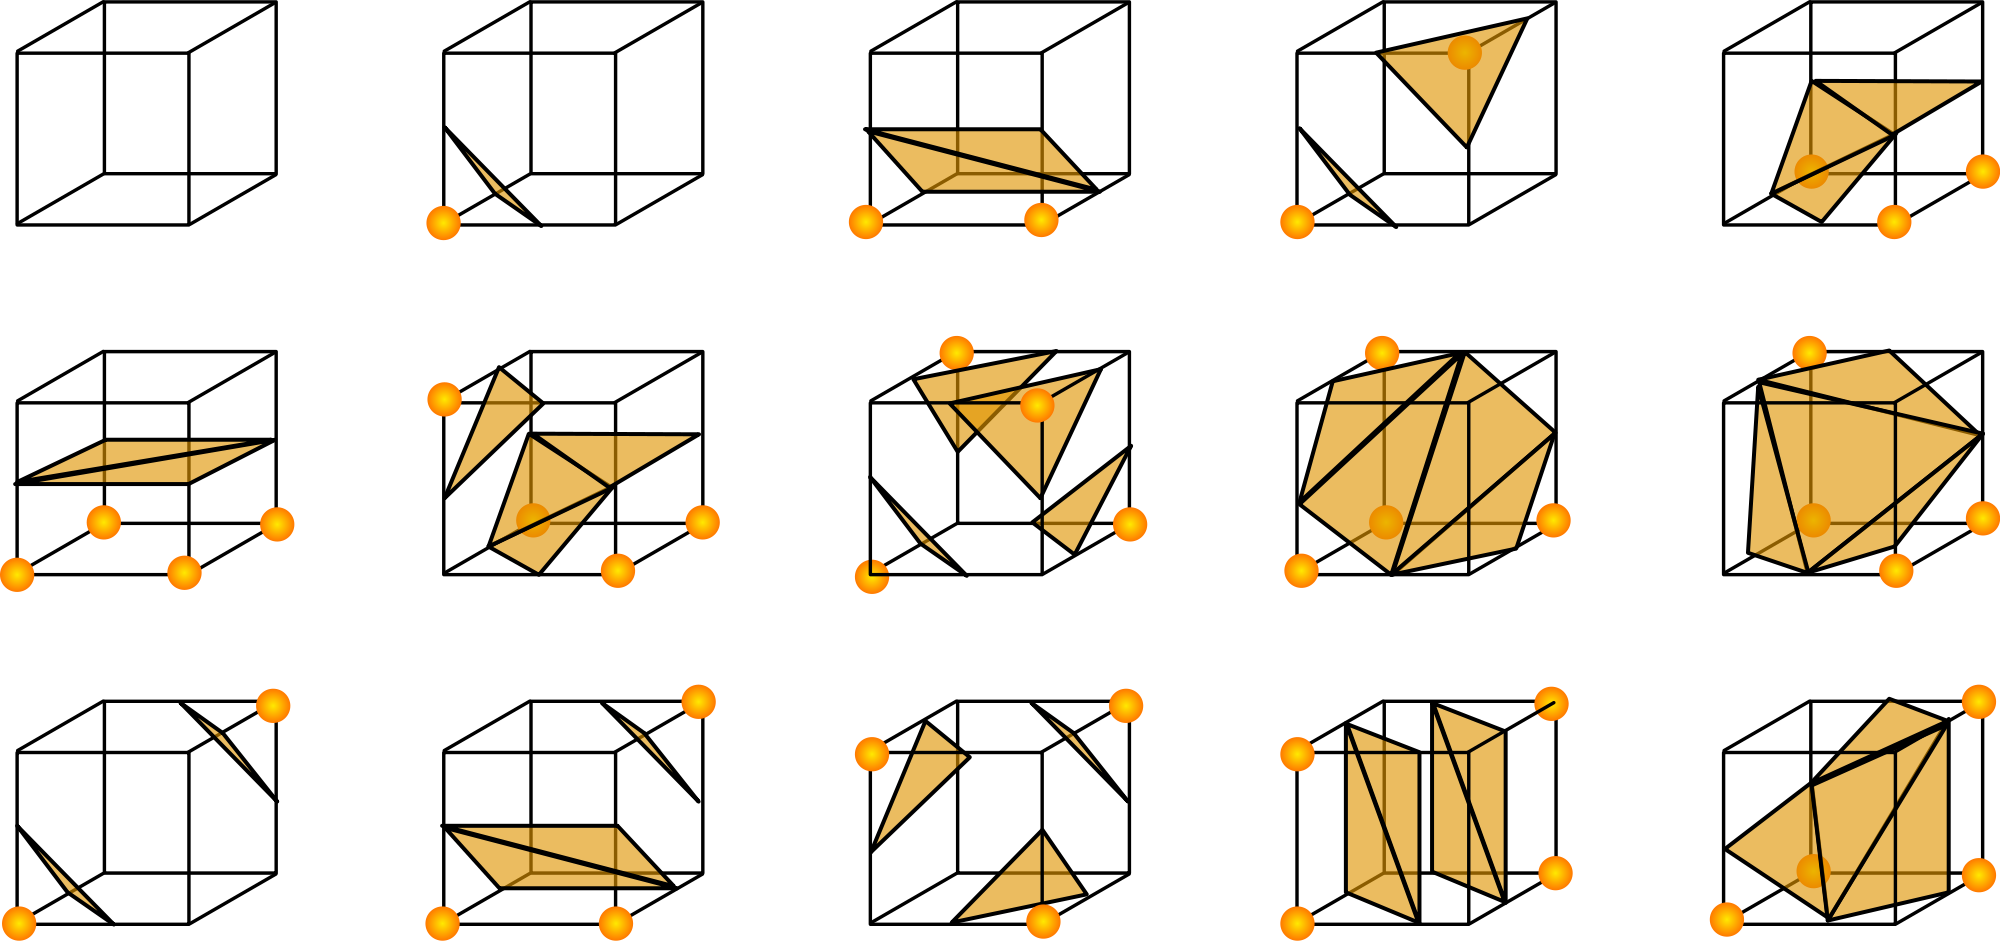
\includegraphics[width=.85\textwidth]{img/mcpolys}
	\caption{Le 15 configurazioni originali di Marching Cubes.}
	\label{fig:mcpolys}
\end{figure}

Marching Cubes ha a disposizione un array di $256$ ($ = 2^{\mbox{\# di vertici di un voxel}}$) possibili configurazioni, che indicano quali vertici sono interni alla mesh e quali sono esterni. Ad ogni vertice è associato un bit in una determinata posizione di un byte, per poter essere trattato come intero. Per ogni vertice viene controllata la sua posizione rispetto alla superficie, e al termine del procedimento, cioè quando si conosce la posizione di tutti i vertici, si ricava la combinazione di configurazioni che meglio approssimano la superficie.

\paragraph{Sviluppi futuri.}
La figura \ref{fig:meshing_octree} mostra che garantire performance $O(1)$ nella cancellazione e nell'aggiornamento di dati costa molto in termini di spazio occupato, in quanto necessita di una lista doppiamente concatenata e, per ciascun voxel salvato, di una coppia di \emph{shared pointer}.
\begin{figure}[htp]
	\centering
	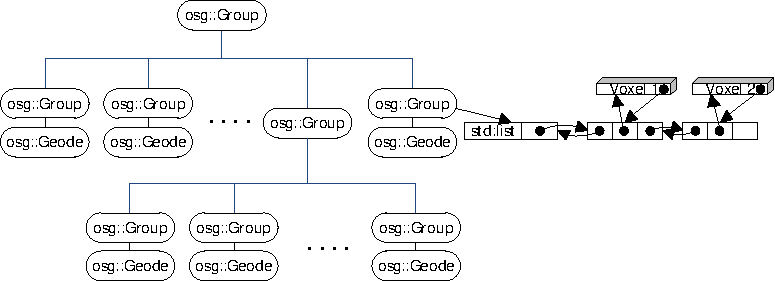
\includegraphics[width=.85\textwidth]{img/meshing_octree}
	\caption{Octree usato dal mesher per visualizzare l'oggetto lavorato.}
	\label{fig:meshing_octree}
\end{figure}

Un possibile sviluppo futuro consiste nel portare le operazioni di cancellazione e aggiornamento a complessità logaritmica, limitando la prima fase a marcare come ``modificate'' quelle liste di voxel interessate dai cambiamenti; sarà poi la seconda fase che si occuperà di riallineare il contenuto dell'albero con lo stato di fatto. Così facendo le liste possono essere sostituite da array e le coppie di puntatori con singoli \emph{weak pointer}\footnote{I concetti di \emph{shared} e \emph{weak pointer} sono mutuati dalla libreria boost e spiegati nella relativa documentazione, reperibile all'url \url{http://www.boost.org/doc/libs/1_52_0/libs/smart_ptr/smart_ptr.htm}} che puntano al voxel, risparmiando così memoria RAM.
